\chapter{Resultados}

\section{Equivalencias entre tipos de datos}

Las equivalencias encontradas entre los tipos de datos FHIR y los tipos de datos openEHR se presentan en el Cuadro \ref{table:equivalents}.

\begin{table}[h]
  \caption{Equivalencias entre tipos de datos}
  \label{table:equivalents}
  \begin{tabular}{l l}
    \hline
    Tipo de dato FHIR &	Tipo de dato openEHR \\
    \hline
    Boolean	& DV\_BOOLEAN \\
    Integer	& DV\_QUANTITY \\
    String	& DV\_TEXT \\
    Decimal	& DV\_QUANTITY \\
    Uri	& DV\_URI \\
    base64Binary	& DV\_PARSABLE \\
    Instant	& DV\_DATE\_TIME \\
    Date	& DV\_DATE \\
    dateTime	& DV\_DATE\_TIME \\
    Time	& DV\_TIME \\
    Code	& DV\_TEXT \\
    Oid	& DV\_URI \\
    id 	& DV\_TEXT \\
    Markdown	& DV\_PARSABLE \\
    unsignedInt	& DV\_QUANTITY \\
    positiveInt	& DV\_QUANTITY \\
    \hline
  \end{tabular}
\end{table}

Cabe mencionar que para todos los tipos de datos FHIR se encuentra su equivalente en openEHR, observándose que ambos estándares comparten los mismos valores de dominio. Los tipos de datos openEHR listados en el Cuadro \ref{table:equivalents}, salvo el tipo DV\_QUANTITY, tienen un atributo value que soporta los valores de sus tipos de datos FHIR equivalentes. El tipo DV\_QUANTITY soporta los valores de sus tipos de datos FHIR equivalentes en su atributo magnitude. Una caso particular es la equivalencia entre el tipo String y el tipo DV\_TEXT. El tipo String puede contener los carácteres Unicode  de tab horizontal, retorno de carro y avance de línea, los cuales no están permitidos en el tipo DV\_TEXT.

Además, se verifica a partir de las especificaciones que las clases de openEHR mantienen sus propósitos.

\section{Arquetipos de Integración}

Las equivalencias entre tipos de datos y el proceso automatizado permiten crear los arquetipos de integración basados en las clases CLUSTER y ELEMENT. Estos arquetipos de integración tienen el propósito principal de ser el punto de entrada de proceso de conversión semántico para importación de datos a sistemas openEHR. La Figura \ref{fig:comparison} muestra de lado a lado un extracto de un arquetipo de integración de paciente creado utilizando el proceso automatizado y el recurso FHIR Paciente del cual se creo.

\begin{figure*}
  \centering
  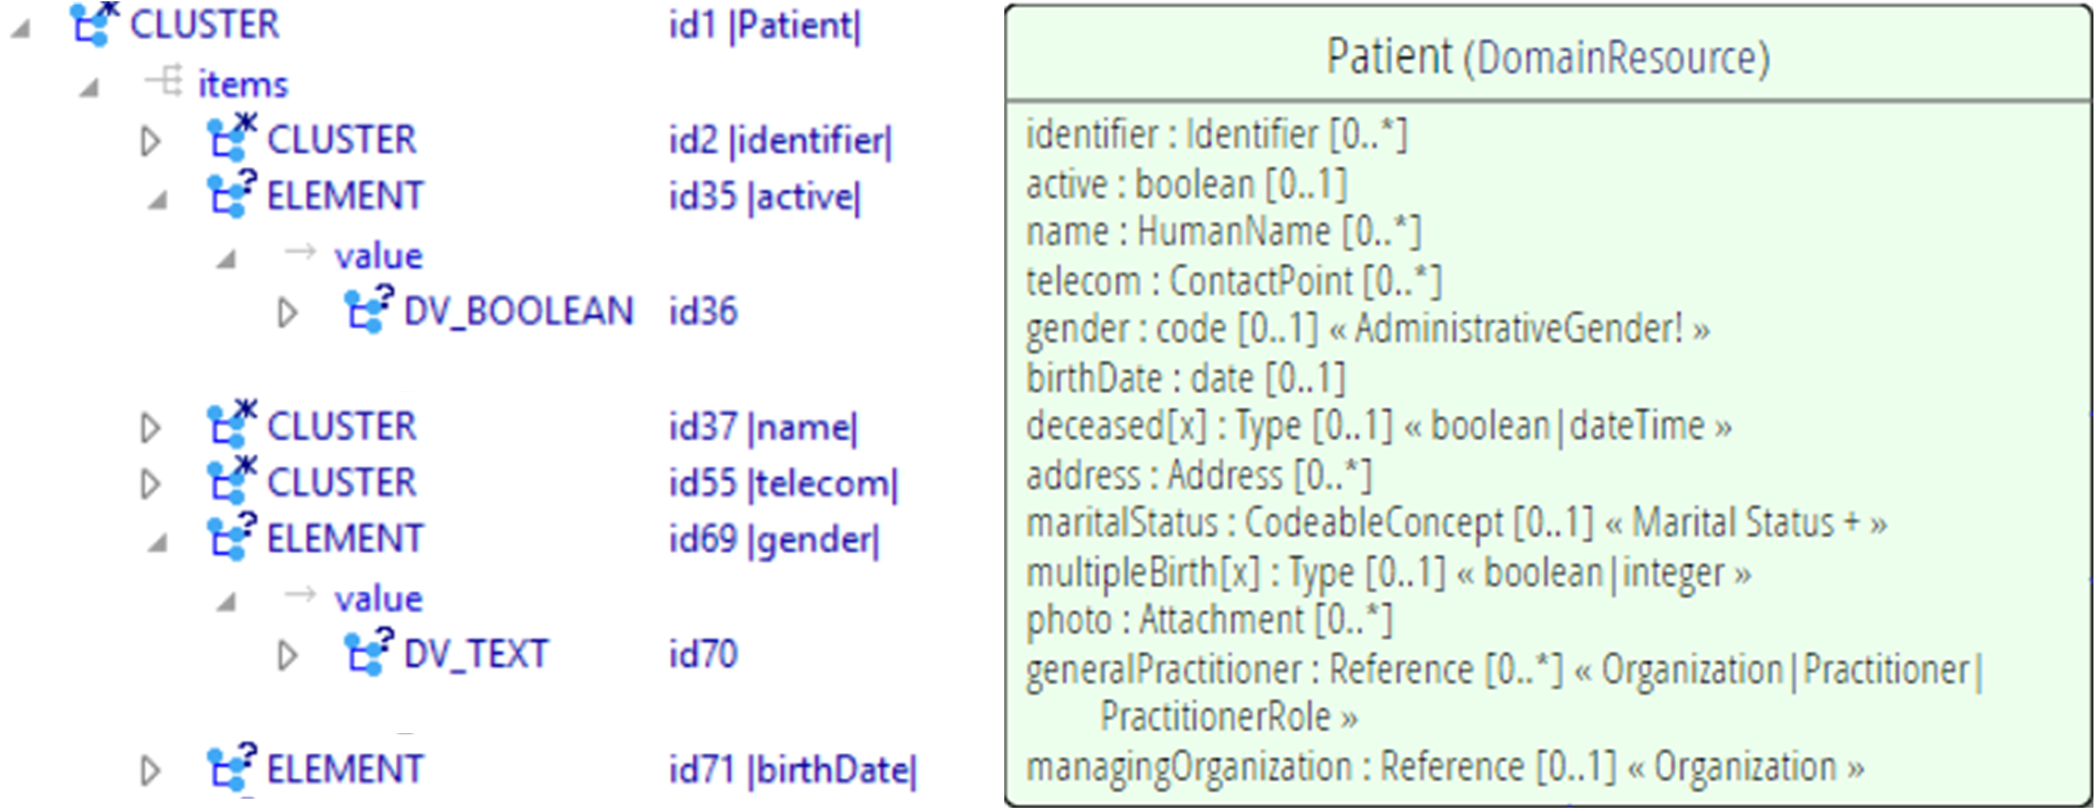
\includegraphics[scale=0.8]{./images/comparison_patient.png}
  \caption{Comparación de un arquetipo de integración de paciente y un recurso de FHIR paciente.}
  \label{fig:comparison}
\end{figure*}

\section{Automatización}

Dentro del atributo snapshot de un recurso FHIR StructureDefinition se encuentra las definiciones de los elementos de un recurso FHR. Un elemento de un recurso FHIR se define en un recurso FHIR ElementDefinition \cite{FHIRElementDefinition}. Tanto los recursos FHIR StructureDefinition y FHIR ElementDefinition tienen representaciones en JSON. Estas representaciones se utiliza en el proceso de automatización para crear un arquetipo openEHR de un recurso FHR de la siguiente forma.

Primero en la etapa de abstracción, el nombre de un recurso FHIR se obtiene del atributo id de un recurso FHIR StructureDefinition. Por cada elemento definido en un recurso FHIR StructureDefinition, se obtiene el nombre del elemento, el tipo del elemento, la cardinalidad mínima y la cardinalidad máxima a partir de los atributos id, type, min y max respectivamente de un recurso FHIR ElementDefinition. Con estos datos se crea una definición de un tipo del elemento con el método descripto más arriba. Una definición de vinculación se crea a partir de un atributo binding de un recurso FHIR ElementDefinition.

Durante la etapa de sustitución, se reemplaza los tipos de datos por sus equivalentes utilizando las equivalencias listadas en el Cuadro \ref{table:equivalents}.

Por último en la etapa de definición, se crea bloques ADL CLUSTER y ELEMENT según explicado más arriba con las siguientes consideraciones. Dado que la clase openEHR DV\_QUANTITY requiere el uso de unidades expresadas en UCUM \cite{UCUM}, se utiliza el valor por defecto de 1 dentro del atributo units para denotar sin unidad. Teniendo en cuenta que la clase openEHR DV\_PARSABLE requiere la especificación del formalismo que utiliza, se emplea los valores base64Binary y Markdown para los tipos FHIR base64Binary y Markdown respectivamente. Un aspecto importante es que definiciones recursivas en recursos FHIR no son soportadas en arquetipos openEHR. Estas definiciones recursivas se limitan a 1 nivel de profundidad en la etapa definición. Una implementación en lenguaje Python de las 3 etapas se encuentra disponible en \cite{PythonImplementation}.

Con el fin de comparar los tiempos de creación manual y automática, se llevó a cabo un experimento en el cual se comparó el tiempo requerido para la creación manual del arquetipo openEHR del recurso SimplePatient presentado en este trabajo  y la creación automática de los arquetipos openEHR de los recursos FHIR categorizados como individuos. Para la creación manual se utilizó el editor ADL WORKbench \cite{ADLWORKbench}. Para la creación automática se utilizó el proceso de la Figura \ref{fig:solution} implementado en el lenguaje Python \cite{PythonImplementation}. Los resultados del experimento mostraron que la creación automática de arquetipos openEHR de todos los recursos categorizados como individuos (6 recursos) tomó en promedio 281.53 ms frente a los 79.5 segundos que tomó en promedio la creación manual de la definición del recurso SimplePatient.
